% Tento soubor nahraďte vlastním souborem s přílohami (nadpisy níže jsou pouze pro příklad)
% This file should be replaced with your file with an appendices (headings below are examples only)

% Umístění obsahu paměťového média do příloh je vhodné konzultovat s vedoucím
% Placing of table of contents of the memory media here should be consulted with a supervisor
%\chapter{Obsah přiloženého paměťového média}

%\chapter{Manuál}

%\chapter{Konfigurační soubor} % Configuration file

%\chapter{RelaxNG Schéma konfiguračního souboru} % Scheme of RelaxNG configuration file

%\chapter{Plakát} % poster

\chapter{The~Design Drafts}
\label{drafts}
This chapter contains complete design drafts of~the~application.

\begin{figure}[!hbt]
	\centering
	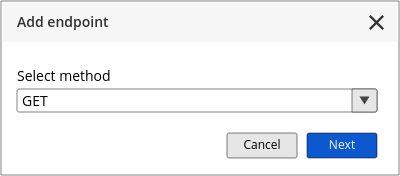
\includegraphics[scale=0.7]{./designs/addTest1.png}
	\caption{Adding endpoint to~a~test case -- selecting the~endpoint's HTTP
	method.}
	\label{figAddTest1}
\end{figure}

\begin{figure}[!hbt]
	\centering
	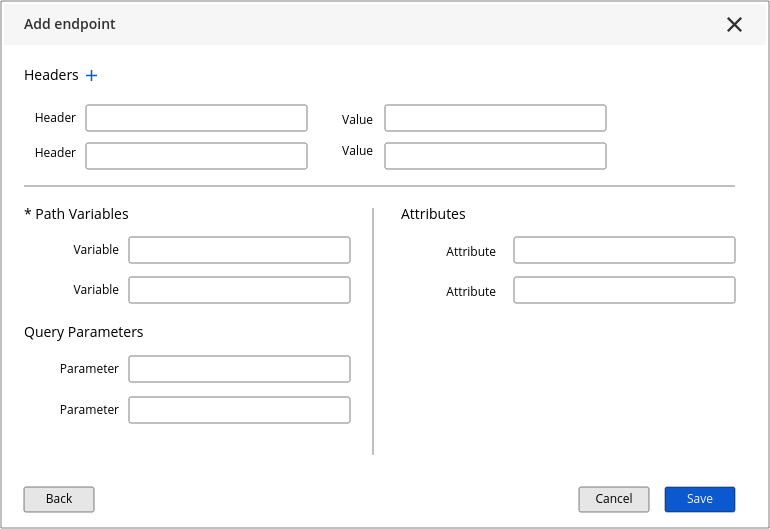
\includegraphics[scale=0.6]{./designs/addTest2.png}
	\caption{Adding endpoint to~a~test case -- form for~filling the~endpoint's
	data.}
	\label{figAddTest2}
\end{figure}


\begin{figure}[!hbt]
	\centering
	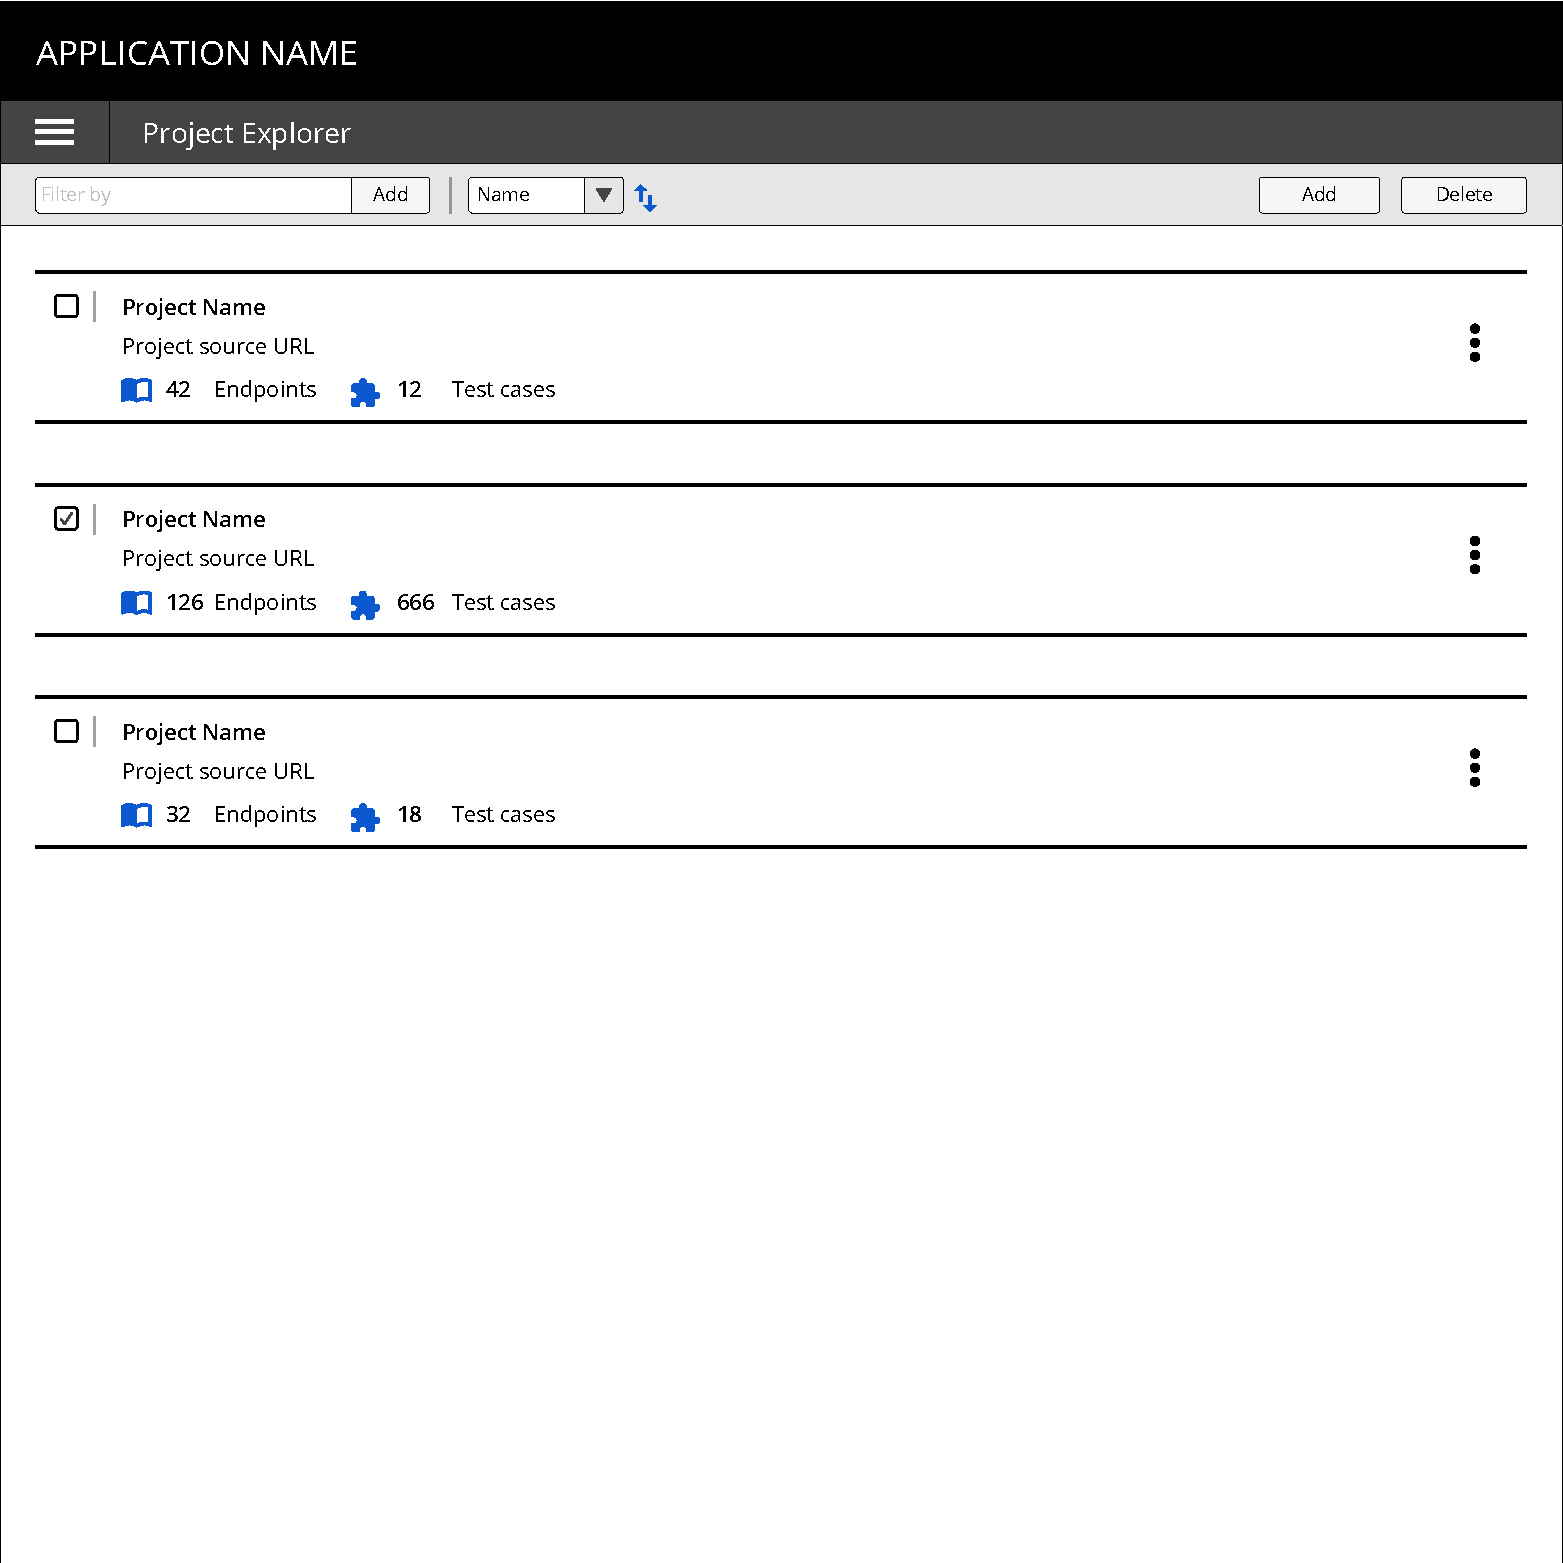
\includegraphics[scale=0.57]{./designs/projectExplorer.pdf}
	\caption{The~Project Explorer page which contains information about projects
	added to~the~application.}
	\label{figExplorerView}
\end{figure}

\begin{figure}[!hbt]
	\centering
	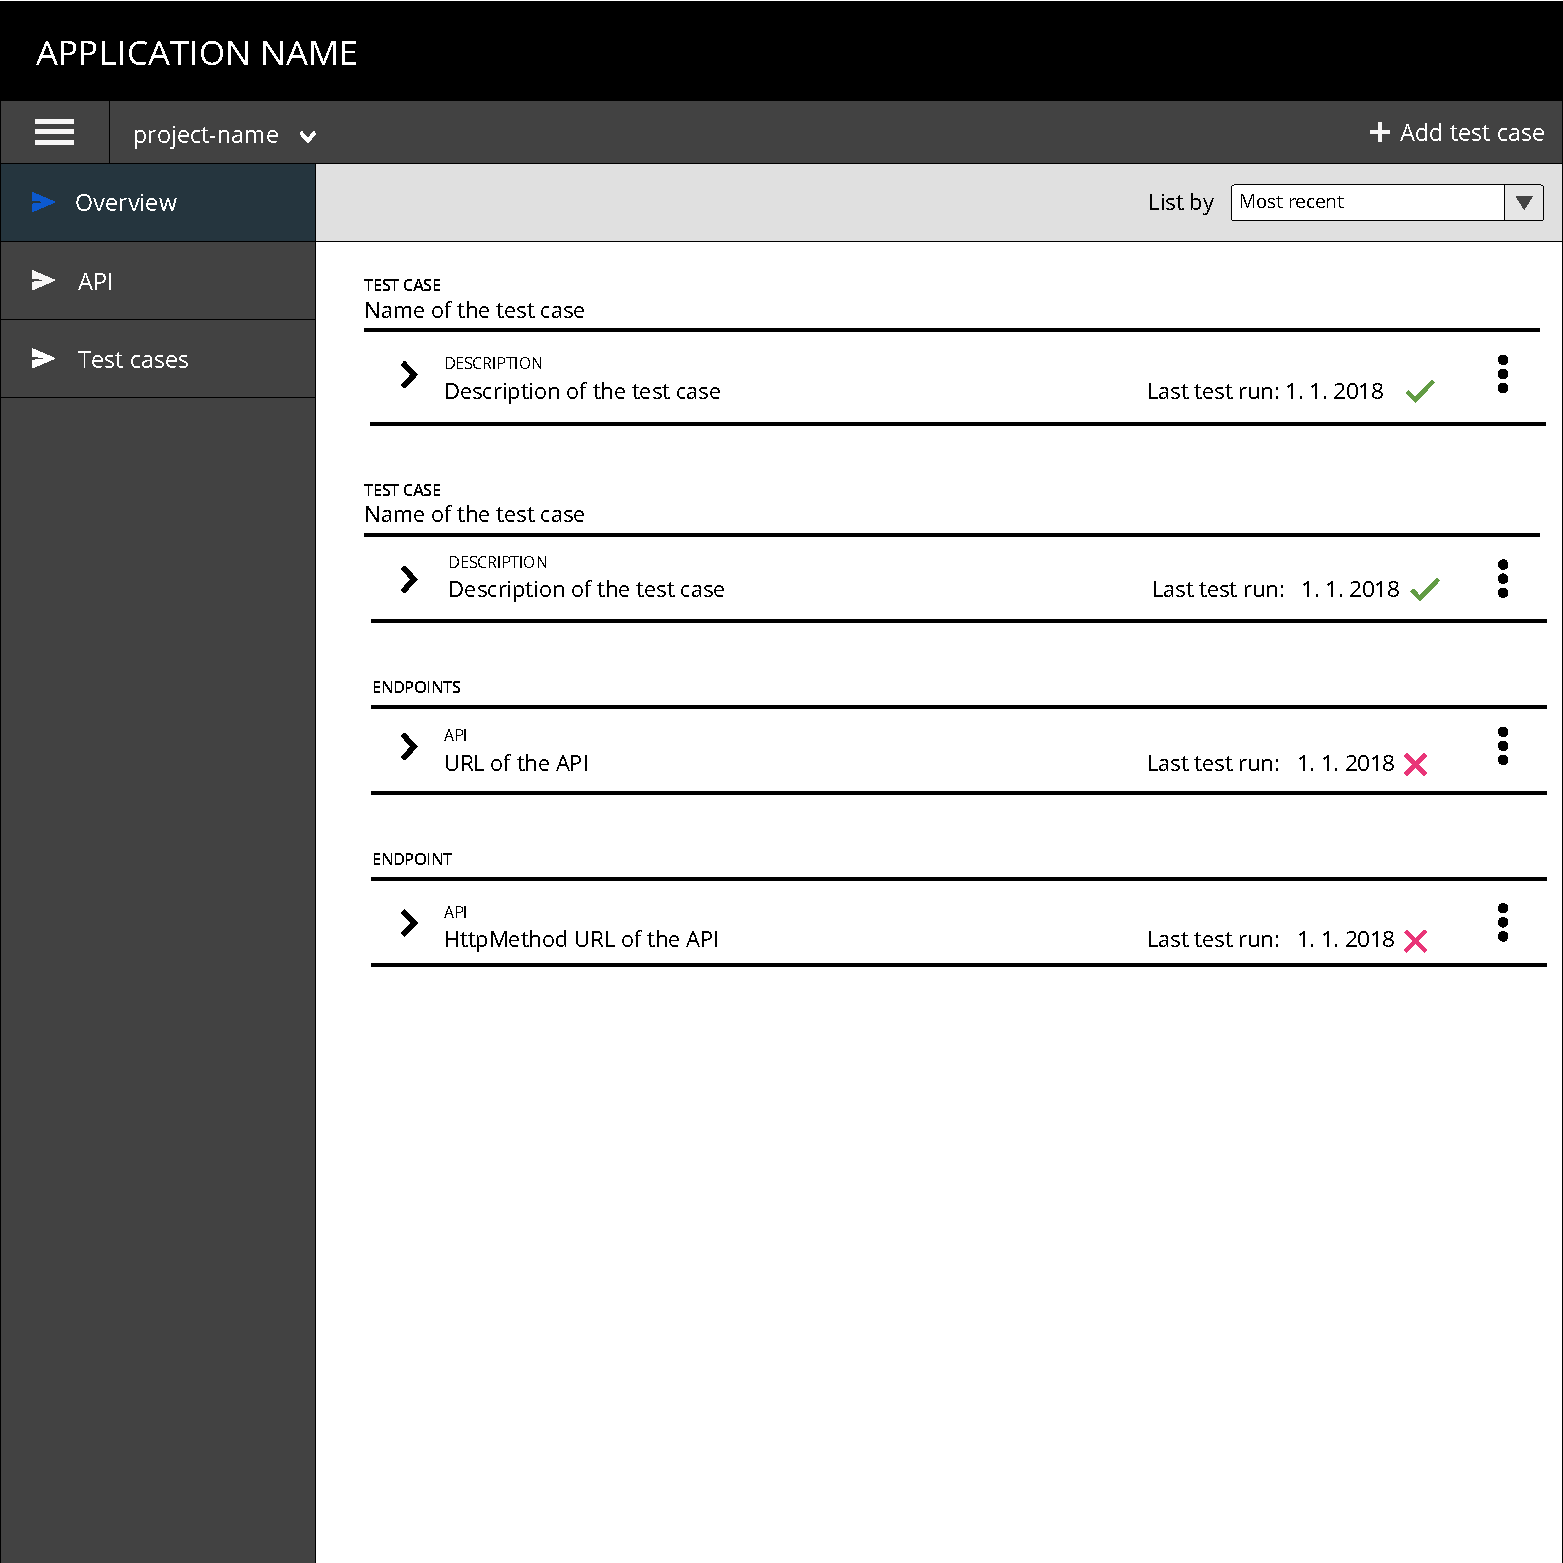
\includegraphics[scale=0.57]{./designs/overview.pdf}
	\caption{The~Dashboard of~the~application that contains recently tested
	endpoints and~test cases.}
	\label{figOverview}
\end{figure}

\begin{figure}[!hbt]
	\centering
	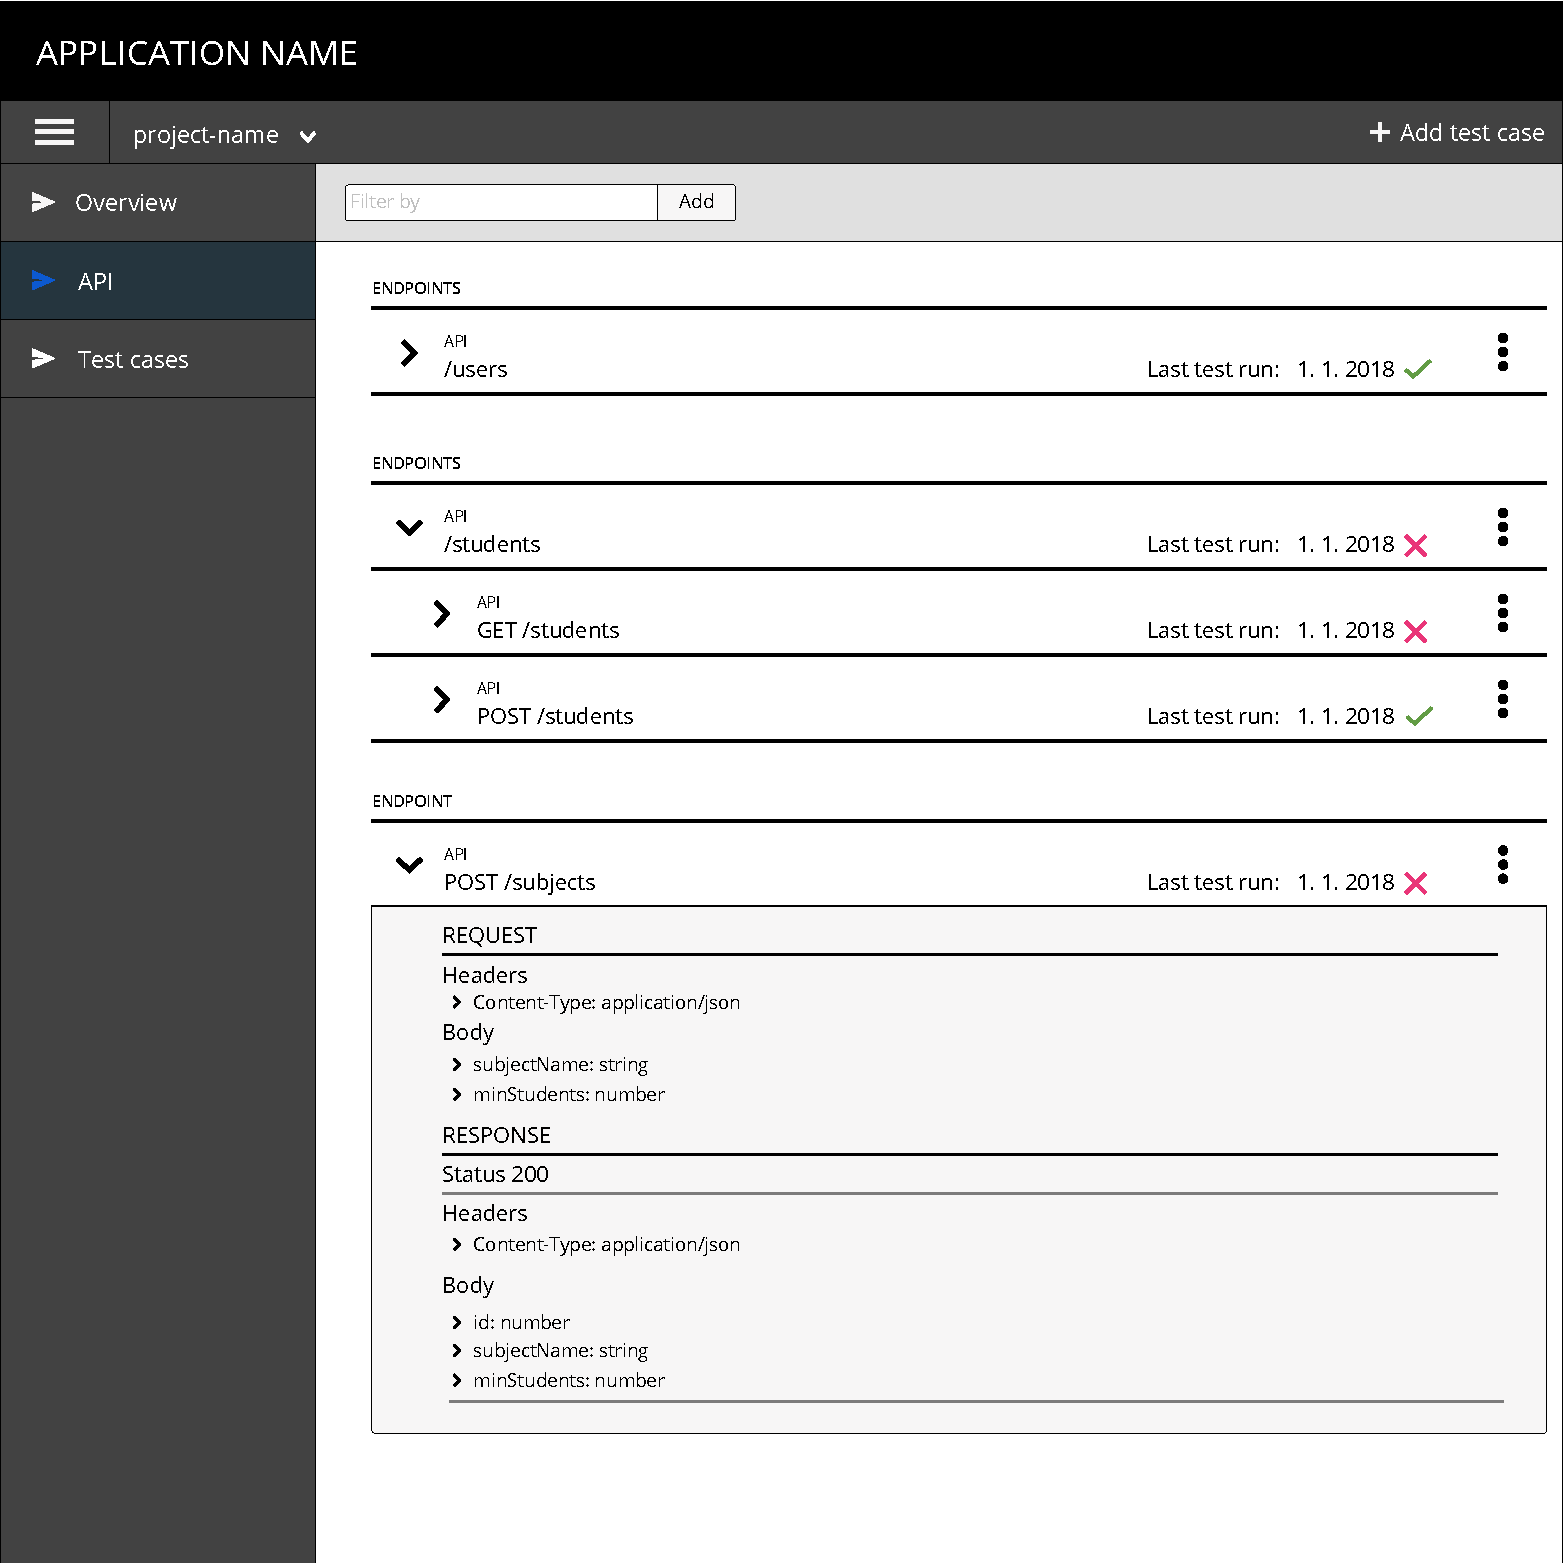
\includegraphics[scale=0.57]{./designs/apiContainer.pdf}
	\caption{The~page with API endpoints ordered into a~hierarchical structure.}
	\label{figAPI}
\end{figure}

\begin{figure}[!hbt]
	\centering
	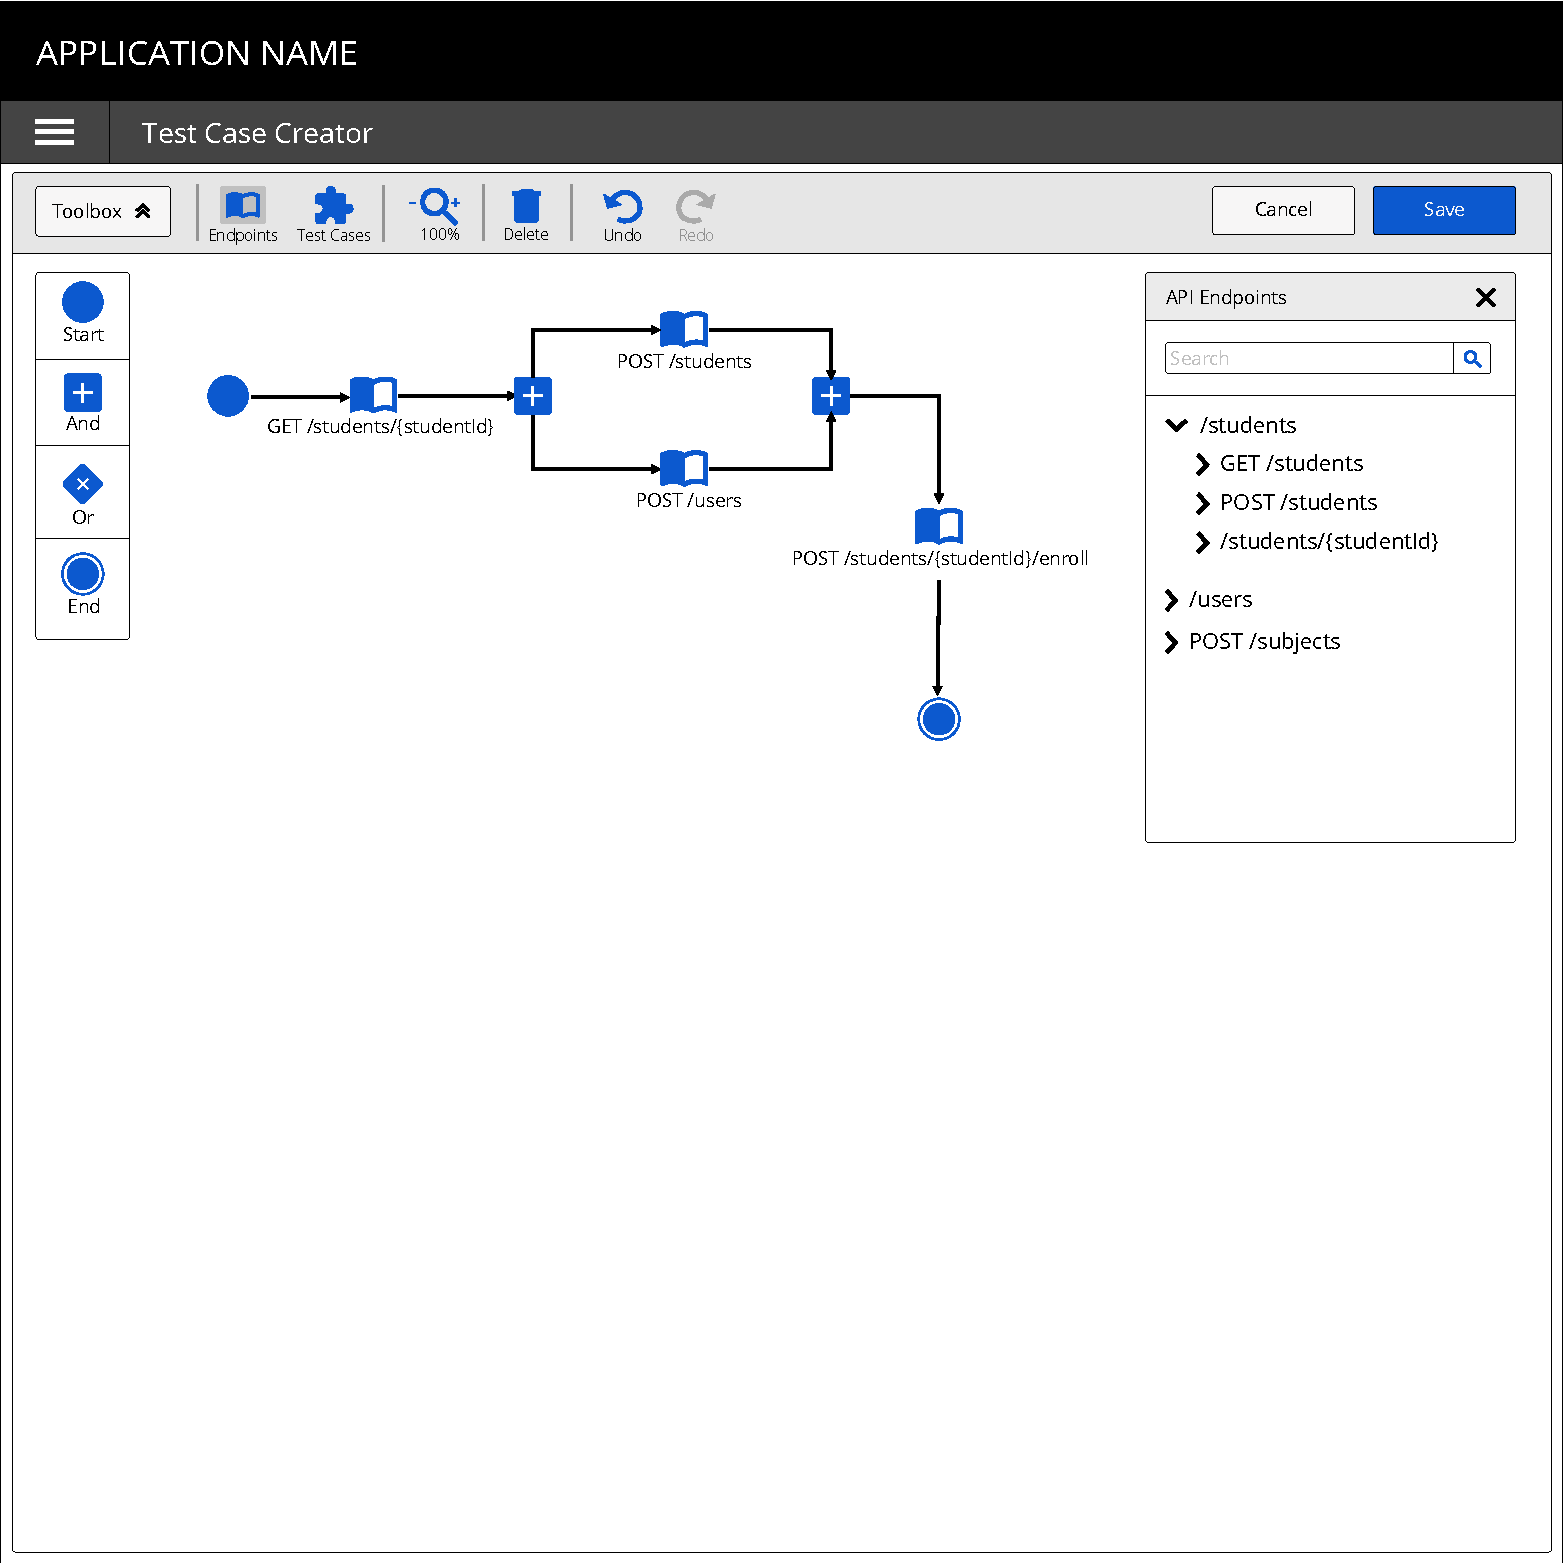
\includegraphics[scale=0.57]{./designs/testCaseCreator.pdf}
	\caption{The~design of~the~Test Case Creator that allows creating test cases
	from~application's API and~other test cases.}
	\label{figCreateTest}
\end{figure}

\begin{figure}[!hbt]
	\centering
	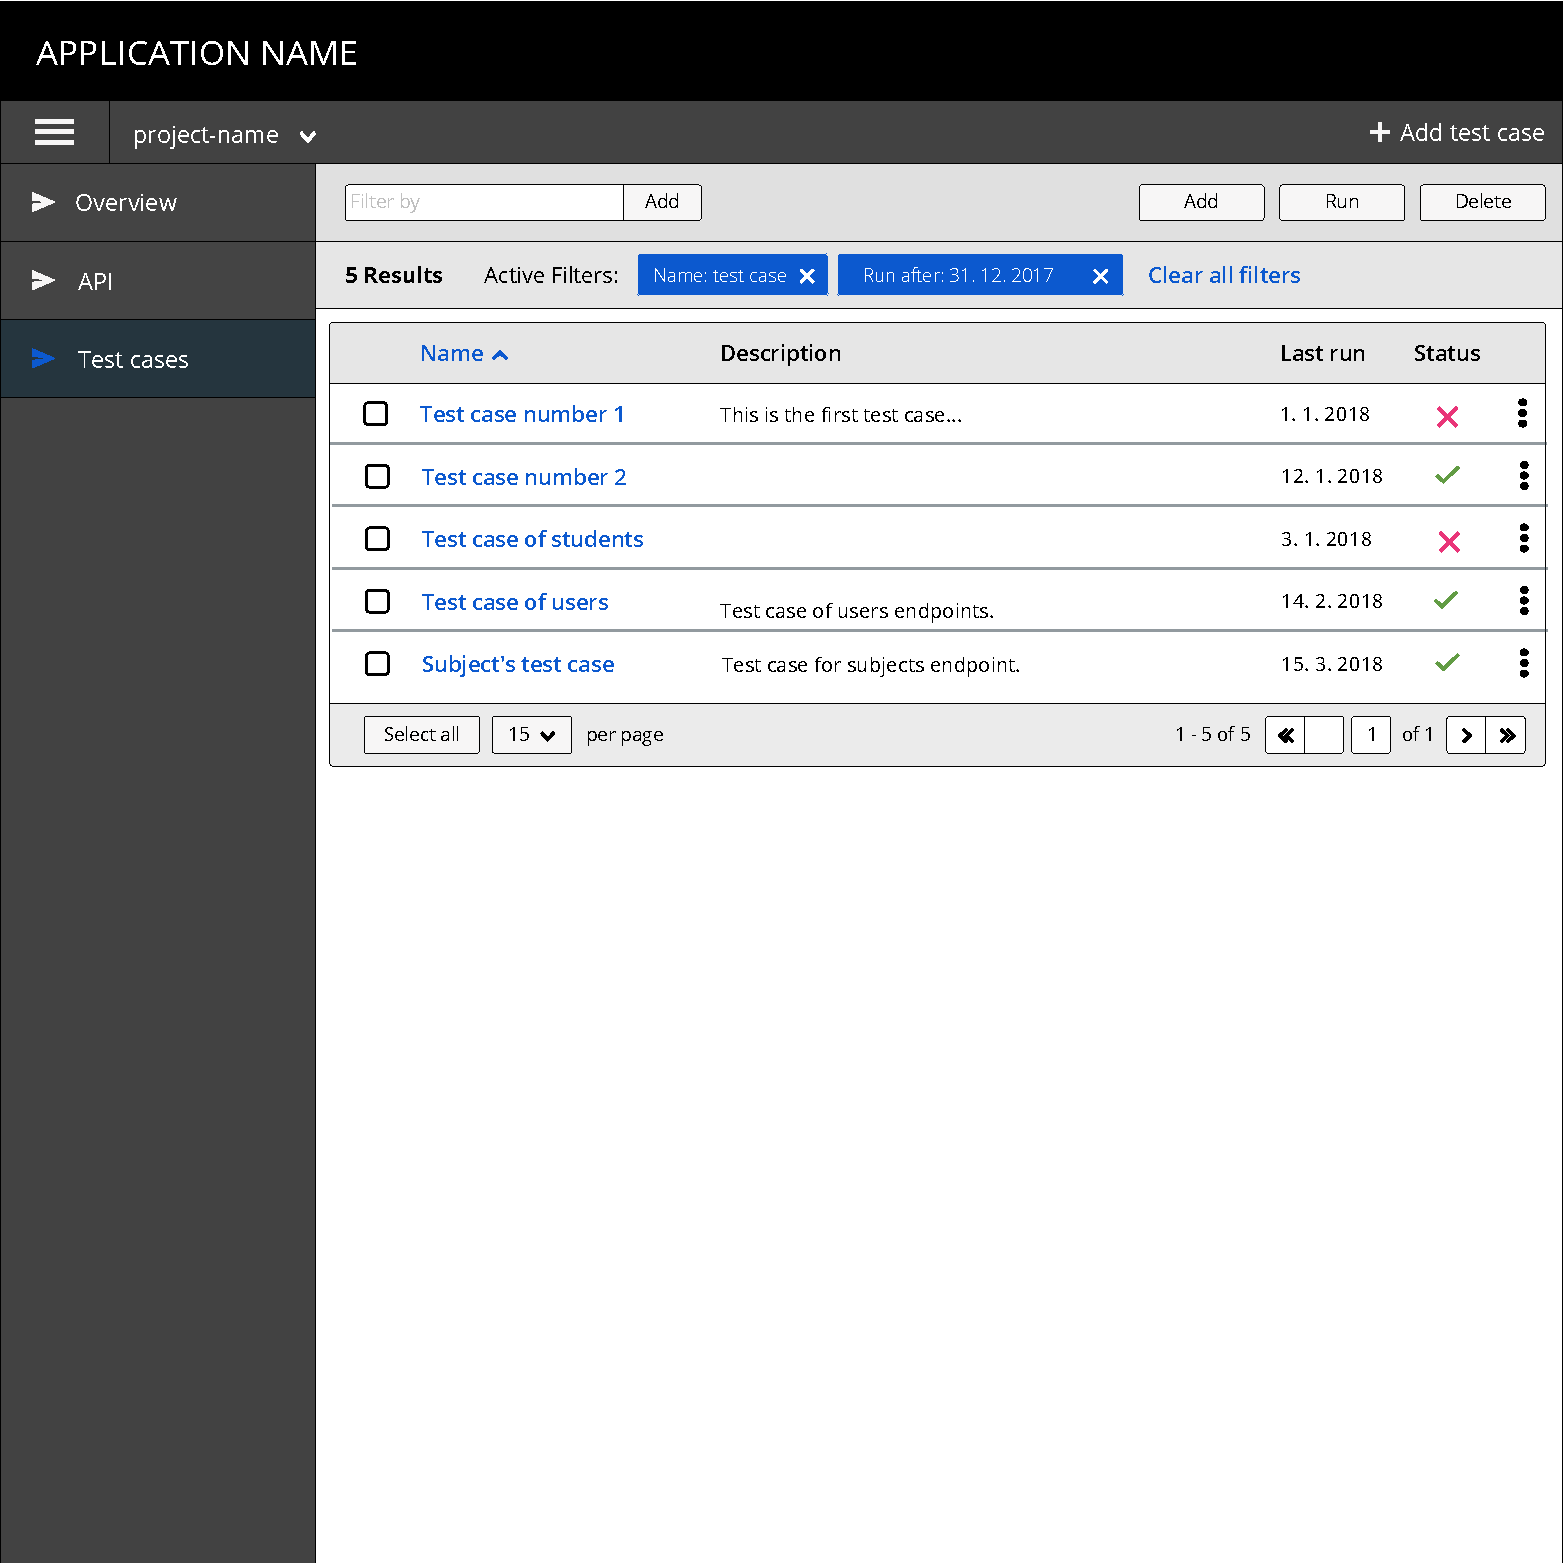
\includegraphics[scale=0.57]{./designs/testCaseContainer.pdf}
	\caption{The~design of~the~test cases overview that contains information about
	created test cases inside a~table.}
	\label{figTestCaseContainer}
\end{figure}

